\documentclass{article} % For LaTeX2e
\usepackage{cos424,times}
\usepackage{hyperref}
\usepackage{url}
\usepackage{graphicx}
\usepackage{caption}
\usepackage{subcaption}
\graphicspath{ {images/} }

\title{Deanonymizing Bitcoin}


\author{
Rob Whitaker\\
Department of Physics\\
Princeton University\\
\texttt{rwhitaker@princeton.edu} \\
\And
Samuel H. Cabot \\
Department of Astrophysics\\
Princeton University \\
\texttt{shcabot@princeton.edu} \\
}

\newcommand{\fix}{\marginpar{FIX}}
\newcommand{\new}{\marginpar{NEW}}

\begin{document}
\setlength{\belowcaptionskip}{-10pt}

\maketitle

\begin{abstract}



.....Graph approaches are better becuase they can use features that represent physical properties.....whatever....sailing is chill.



\end{abstract}

\section{Introduction}

Since several years ago, we have lived in the epoch of crytocurrency: decentralized, digitial forms of payment with encryption at their cores. Its adoption was catalyzed by a clever solution to the double-spending problem (the use of the same currency for multiple transactions): Bitcoin \cite{Nakamoto2008}. A public ledger (blockchain) hashes and stores every transaction made with the currency. Its allure and subsequent popularity, however, is perhaps attributed to its anonymity. Transactions never demand the identification of either the vendor or customer. Hence increased privacy concerns in our daily lives have driven the rise of Bitcoin. One side effect is the security it provides to criminals including, for example, sellers of illicit goods (Silk Road \cite{Christin2013}), and hackers (Ransomware \cite{Pathak2016}). Authorities may therefore seek ways to undermine the privacy granted by bitcoin in efforts against such threats.

One approach is identification of latent structure within the available bitcoin transaction data. While actual names are not recorded, the blockchain tracks spenders and recievers through addresses linked their virtual wallets. Patterns can be extracted from these entries (e.g. an address that conistently recieves payments is likely an organized vendor). This paper uses machine learning techniques to make predictions of transactions by training on a one-year time interval of blockchain data, and hence tests the viability of different algorithms to identify underlying information in massive yet sparse datasets.

\section{Data and Methods}

Our dataset consists of pairs of sending and receiving addresses and the number of interactions between them over a time span from March 2012 to March 2013 (corresponding to blocks 170000 to 225000). There are 444,075 addresses and 3,348,026 recorded pairs. The number of possible transactions ($\sim 2 \times 10^{11}$) yields a sparsity of $\sim 10^{-5}$. We seek to train our models on this data to predict whether a pair of addresses will have a transaction in the future. We take two distict approaches. The first is factorization of the blockchain sparse matrix, which lets us identify eigenvalues representative of the strongest transaction patterns. The second is a graph-based analysis, in which we derive features from nodes and edges corresponding to addresses and transactions. These are two prominent and well-studied techniques, and therefore serve as the foundation of our analysis.

\subsection{Matrix Factorization Methods}

Factorization (Decomposition) of a matrix involves numerically approximating it as a product of two or more matrices which contain feature information. One may set a small number of features to significantly reduce dimensionality of the component matrices, which is extremely useful since it extracts the strongest latent signals from otherwise noisy data and improves prediction accuracy. We test two decomposition models that support sparse matrices. 
\textbf{Singular Value Decomposition} (SVD) determines three component matrices. The outer two are unitary and are comprised of basis vectors. The central one is diagonal and contains the singular values.
\textbf{Non-negative Matrix Factorization} (NMF) assumes a non-negative input matrix, and determines two constituent matrices by minimizing the Frobenius norm \cite{scikit-learn}. Thus vectors are always superpositions of the components. These models are summarized in Figure~\ref{fig:matrix}.




\subsection{Graph Feature Extraction}

Lorem Ipsum.

\subsubsection{Classification Methods}

Use different classifiers for graph feature modeling

%Intuition indicates that regression may be a useful approach to the methylation imputation problem, so we survey a breadth of different regressors from the scikit-learn libraries \cite{scikit-learn}.

\begin{itemize}
	\item \textbf{Tree} \hspace{3.5pc}: \textit{(DT) Decision Tree (of depth 10)}
	\item \textbf{Tree} \hspace{3.5pc}: \textit{(ET) Extra Trees Regressor (of depth 10)}
 	\item \textbf{Linear model}\hspace{0.5pc}: \textit{(LR) Linear Regression}
	\item \textbf{Linear model}\hspace{0.5pc}: \textit{(RR) Ridge Regression}
	\item \textbf{Neighbors} \hspace{1.125pc} : \textit{(KNN) K Neighbors Regressor}
	\item \textbf{Ensemble}\hspace{1.5pc} : \textit{(RF) Random Forest Regressor}
	\item \textbf{SVM} \hspace{3pc} : \textit{(SVR) Support Vector Regression}
\end{itemize}


%As described in the scikit-learn documentation \cite{scikit-learn}, different modeling schemes underlie each of these regression types: Trees (DT) are based on learning rules from the data through decision trees; these can be randomized (ET) or applied to many subsets (RF). Neighbor methods (KNN) use neighboring data points and clustering/sparsity information to make predictions. Support vector machines (SVM) classify through separation of data. Generalized linear models (LR) seek least squares; this can be modified to impose penalties (RR). All of the classifiers return informative statistics, which enables straightforward comparison of performance. 

\section{Results}

\subsection{Decomposition True Positive Rates}

Here we present the performance of our two matrix decomposition methods, SVD and NMF. We also compare them against 'Random,' in which the component matrices are randomly generated with elements in [0, 1]. Both of the decomposition methods perform much better than the random case, as summarized in Figure~\ref{fig:matrix}. NMF performs the best consistently, perhaps because of the non-negative assumption. It successfully identifies transactions at a true positive rate of 0.51, with an erroneous false positive rate of only 0.1. Both models however are far from optimal binary classification (a point at FPR = 0, TPR = 1). 


\begin{figure}[!h]

%\begin{table}[h]%
\begin{minipage}[b]{0.45\linewidth}
\centering

\begin{footnotesize}
\setlength{\tabcolsep}{5pt}
\renewcommand{\arraystretch}{2.85}
\begin{tabular}[b]{c c c c | c c}
    \hline
    Name & Formula & $N_{comp}$ & tol & ROC & TPR$_{{\rm FPR = } 0.1}$\\
    \hline
    {\it SVD} & $\mathbf{ X = USV}$ & 10 & $10^{-10}$ & 0.64 & 0.39 \\
    {\it NMF} & $\mathbf{ X = WH}$ & 20 & $10^{-10}$ & 0.74 & 0.51 \\
    {\it Random} & $\mathbf{ X = R^{1}R^{2}}$ & 10 & N/A & 0.50 & 0.10 \\
    \hline
\end{tabular}
\end{footnotesize}
%\caption{Table}

%\end{table}
\end{minipage}
\begin{minipage}[b]{0.8\linewidth}


\centering
  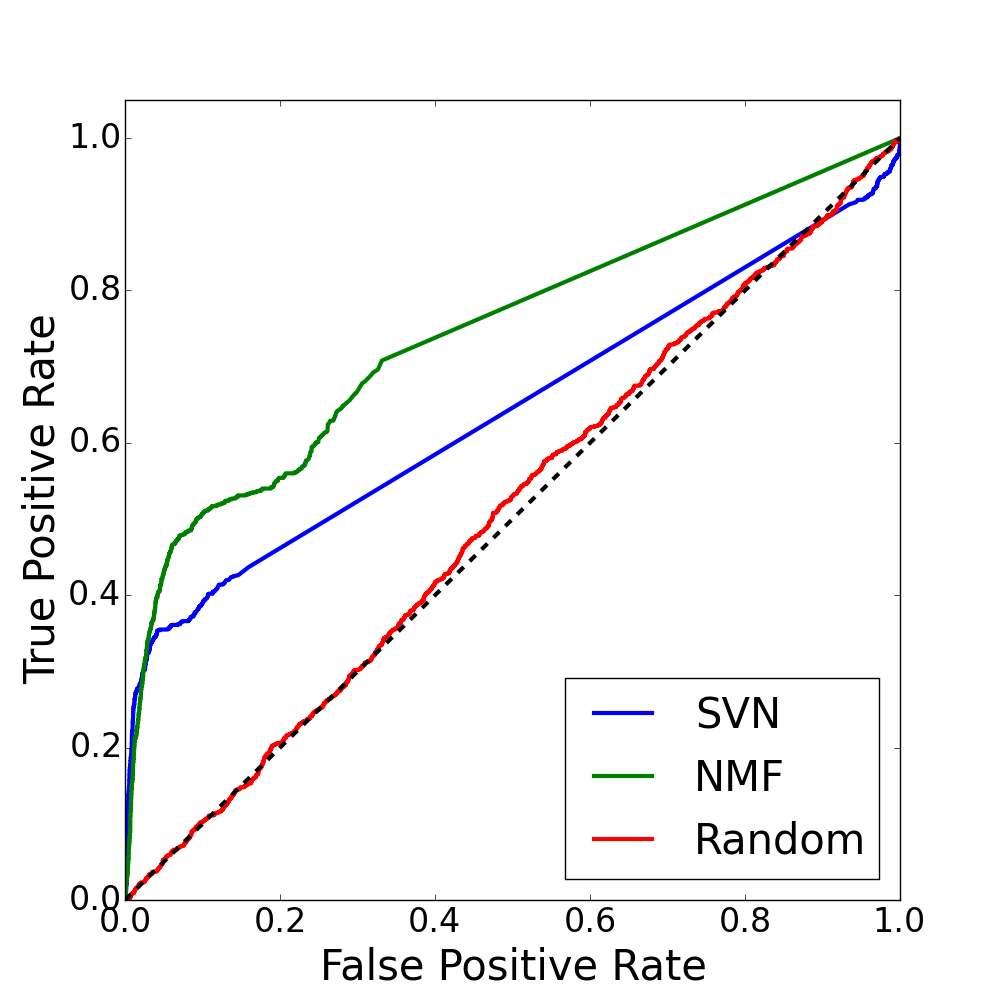
\includegraphics[width=0.45\textwidth]{ROC.png}
%  \caption{Receiver Operating Characteristic curves for each of the models.}
  \label{fig:roc}
\end{minipage}

\caption{Properties of matrix decomposition models including name, formulation, number of components (reduced dimension), and tolerance level. Also performance including ROC area and true positive rate with at most 0.1 false positive rate. Parameters were chosen for a balance of run-time and accuracy.}
\label{fig:matrix}
\end{figure}



%\pagebreak

\subsection{Graph Classifier Performance}


Graphs are cool.

\begin{figure}
\centering
  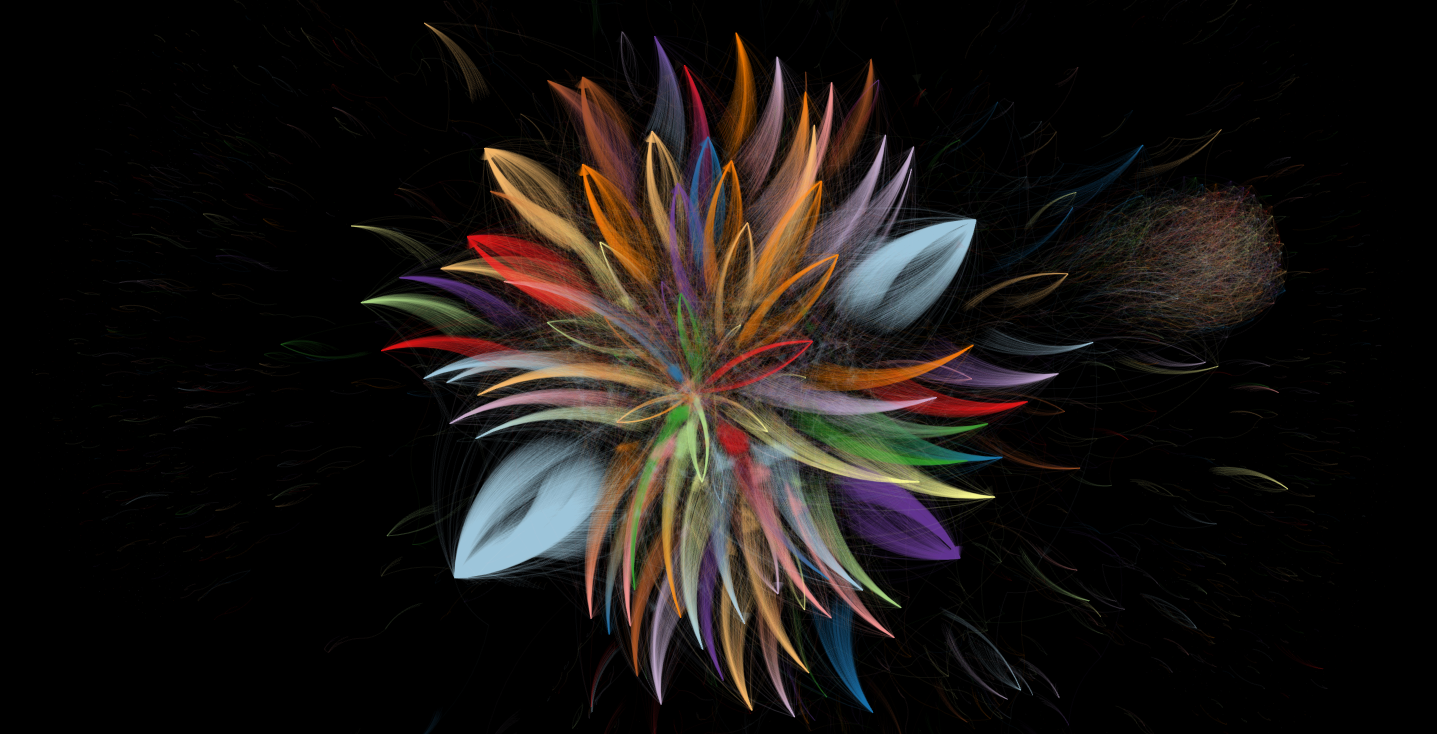
\includegraphics[trim={9cm 0 3cm 0},clip, width=0.75\textwidth]{50000visualization.png}
%  \caption{Receiver Operating Characteristic curves for each of the models.}
\caption{Visualization of 50000 randomly selected transactions. The most active nodes are clearly visible. Connections between these hubs and smaller nodes provide the basis for our graph analysis.}
  \label{fig:vis}
\end{figure}


\section{Discussion and Conclusion}


Lorem Ipsum



%\subsubsection*{Acknowledgments}
%We would like to thank the course staff and instructors for their invaluable %assistance.

\bibliography{ref}
\bibliographystyle{IEEEtran}
\end{document}
